\section{Deep Reinforcement Learning}
\begin{figure}[!h]
    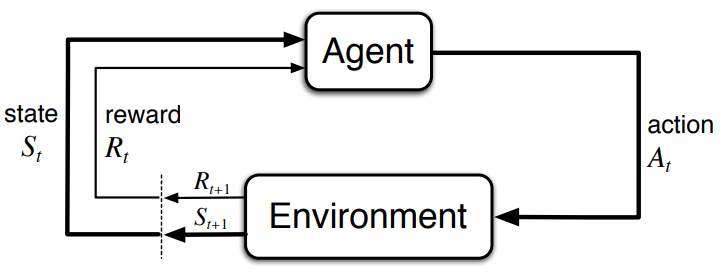
\includegraphics[width = 0.8\columnwidth]{figures/DeepReinforcementLearning/EnvironmentAgent.png}
\end{figure}

Agent learns from experience provided by a simulation of a environment.
The Goal is to maximize the expected cumulative reward/return.
cumulative reward or return (G):
\[
G_t = R_{t+1} + R_{t+2} + R_{t+3} + \dots + R_T
\]
Dicounted return:
\[
G_t = R_{t+1} + \gamma R_{t+2} +\gamma^2 R_{t+3} + \dots = \sum_{k=0}^{\infty}\gamma^k R_{t+k+1}
\]
\begin{figure}[!h]
    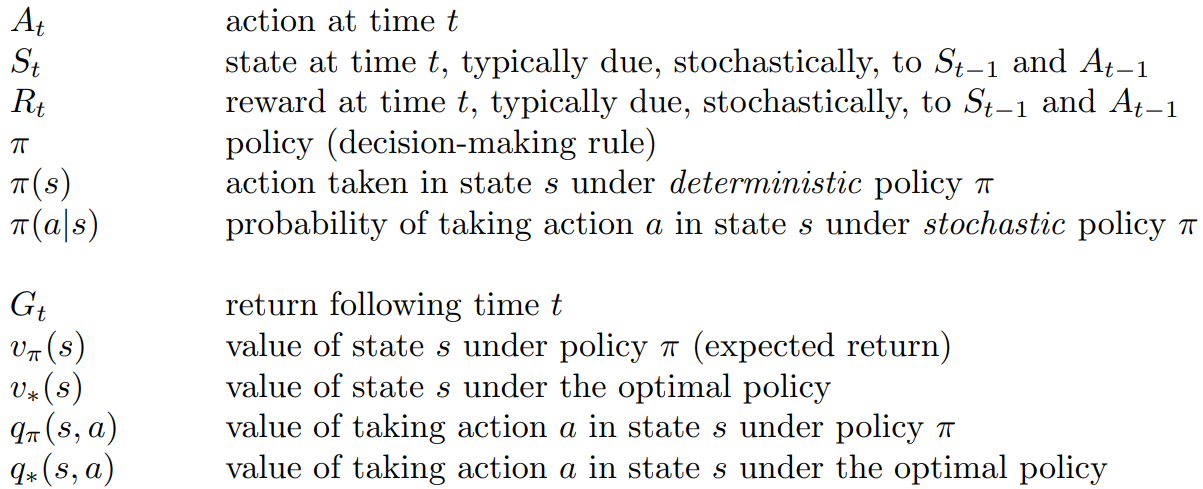
\includegraphics[width = \columnwidth]{figures/DeepReinforcementLearning/OverviewNotation.png}
\end{figure}
\subsection{Mehtods Overview}
\begin{figure}[!h]
    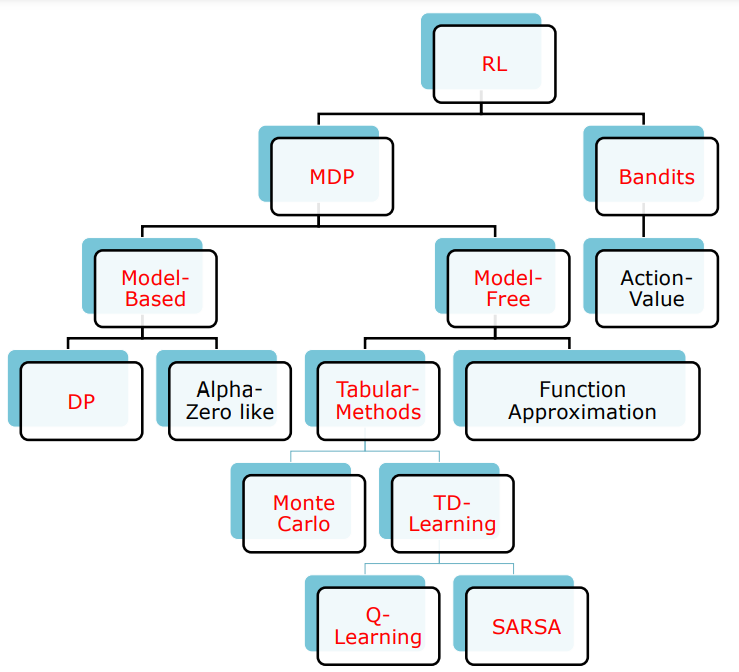
\includegraphics[width = \columnwidth]{figures/DeepReinforcementLearning/RLOverview.png}
\end{figure}
\subsubsection{Value based methods}
\begin{itemize}
    \item \textbf{Monte-Carlo Methods:} Estimate the returns from the rewards collected during the episode.Value estimation and policies are only changed \textbf{on the completion} of an episode

    \item \textbf{Time-Difference Methods:} Estimate the returns from the rewards and the approximated
    returns of the next step(s)
\end{itemize}
\begin{figure}[!h]
    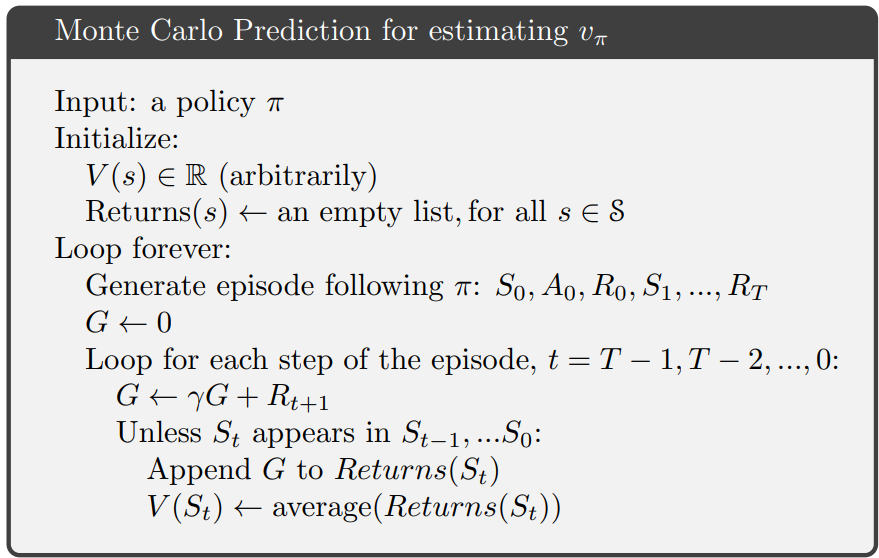
\includegraphics[width = \columnwidth]{figures/DeepReinforcementLearning/MonteCarlo.png}
\end{figure}


